\section{Experiments}

In this section we discuss the performance of our proposed LSA algorithm on randomly generated instances with density less than the threshold and then on real-world large datasets with arbitrary densities.
 The rationale of our evaluation is two-fold. First, we establish the effectiveness of LSA for randomly generated instances with densities close to the threshold in terms of abstract cost measures and compare it with the state of the art method employed for Cuckoo Hashing for a large number of randomly generated instances. Second, we would want to validate the performance of LSA in terms of wall-clock times on large real-world bipartite graphs with arbitrary densities and structure ( i.e. these are not necessarily left regular bipartite graphs). 
 
\subsection{Performance on Random Graphs}

We present some simulations to compare the performance of local search allocation with the random walk method which (to the best of our knowledge) is currently the state-of-art method and so far considered to be the fastest algorithm for the case $k\ge 3$. We recall that in the random walk method we choose a location at random from among the $k$ possible locations to place the item. If the location is not free, the previous item is moved out.  The moved out item again chooses a random location from among its choices and the procedure goes on till an empty location is found. In our experiments we consider $n\in [10^5, 5\times 10^6]$ locations and $\lfloor cn \rfloor$ items. The $k$ random locations are chosen when the item appears. All random numbers in our simulations are generated by \emph{MT19937} generator of GNU Scientific Library~\cite{gnu}. 

Recall that a move is either placing an item at a free location or replacing it with other item. 
In Figure~\ref{fig:1} we give a comparison of the total number of moves (averaged over $100$ random instances) performed by local search and random walk methods for $k=3$ and $k=4$. Figure~\ref{fig:2} compares the maximum number of moves (averaged over $100$ random instances) for a single insertion performed by local search and random walk methods. Figure~\ref{fig:3} shows a comparison when the number of items are fixed and density (ratio of number of items to that of locations) approaches the threshold density. Note that the time required to obtain an allocation by random walk or local search methods is directly proportional to the number of moves performed. 
\begin{figure*}[h!]
   \centering  
     \subfigure[$k=3$, $c=0.90 ~(c^*_3\approx 0.917)$]{\label{fig:total}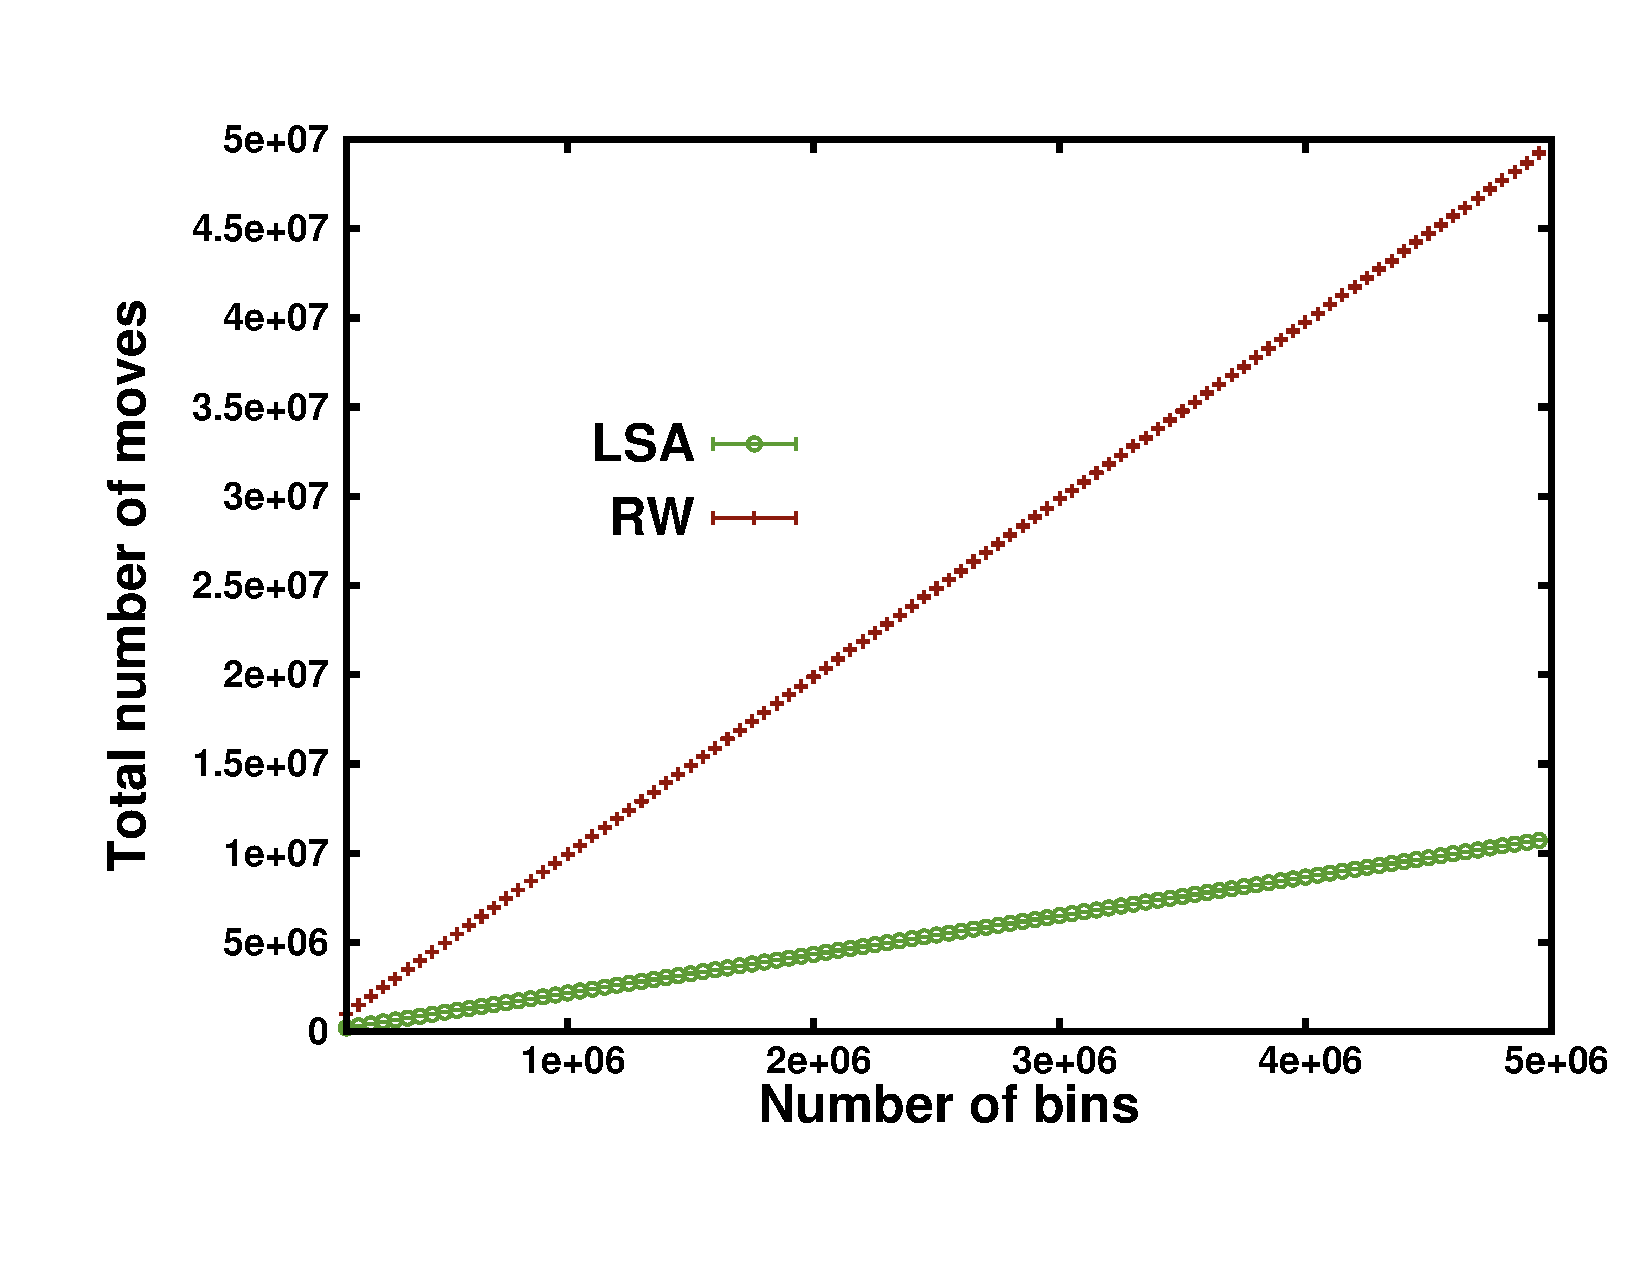
\includegraphics[width=0.45\textwidth]{total-3.pdf}}
   \quad
     \subfigure[$k=4$, $c=0.97 ~(c^*_4\approx 0.976)$] {\label{fig:all-3}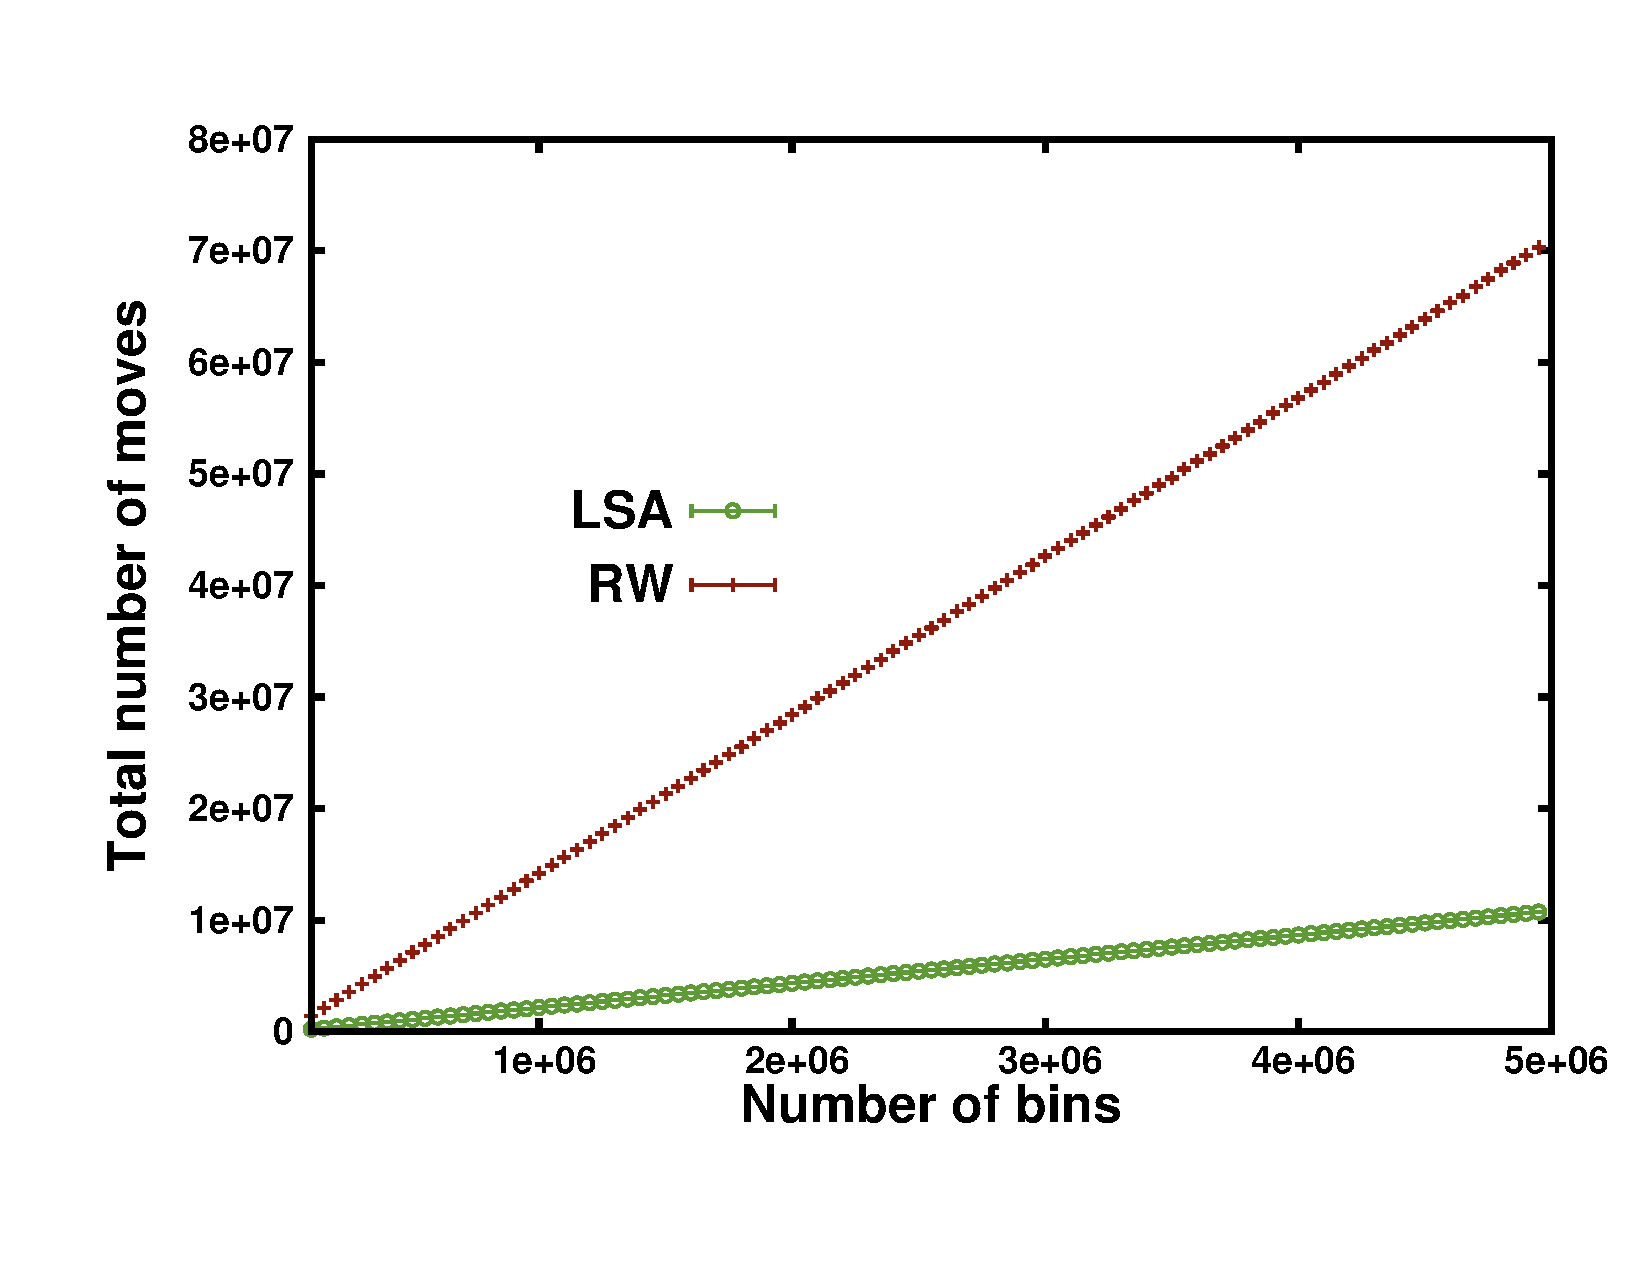
\includegraphics[width=0.45\textwidth]{total-4.pdf}}
     \vspace{-8pt}
   \caption{Comparison of total number of moves performed by local search and random walk methods.}
   \label{fig:1}
\end{figure*}
\begin{figure*}[h!]  
   \centering  
    \subfigure[ $k=3$, $c=0.90 ~(c^*_3\approx 0.917)$.]{\label{fig:max}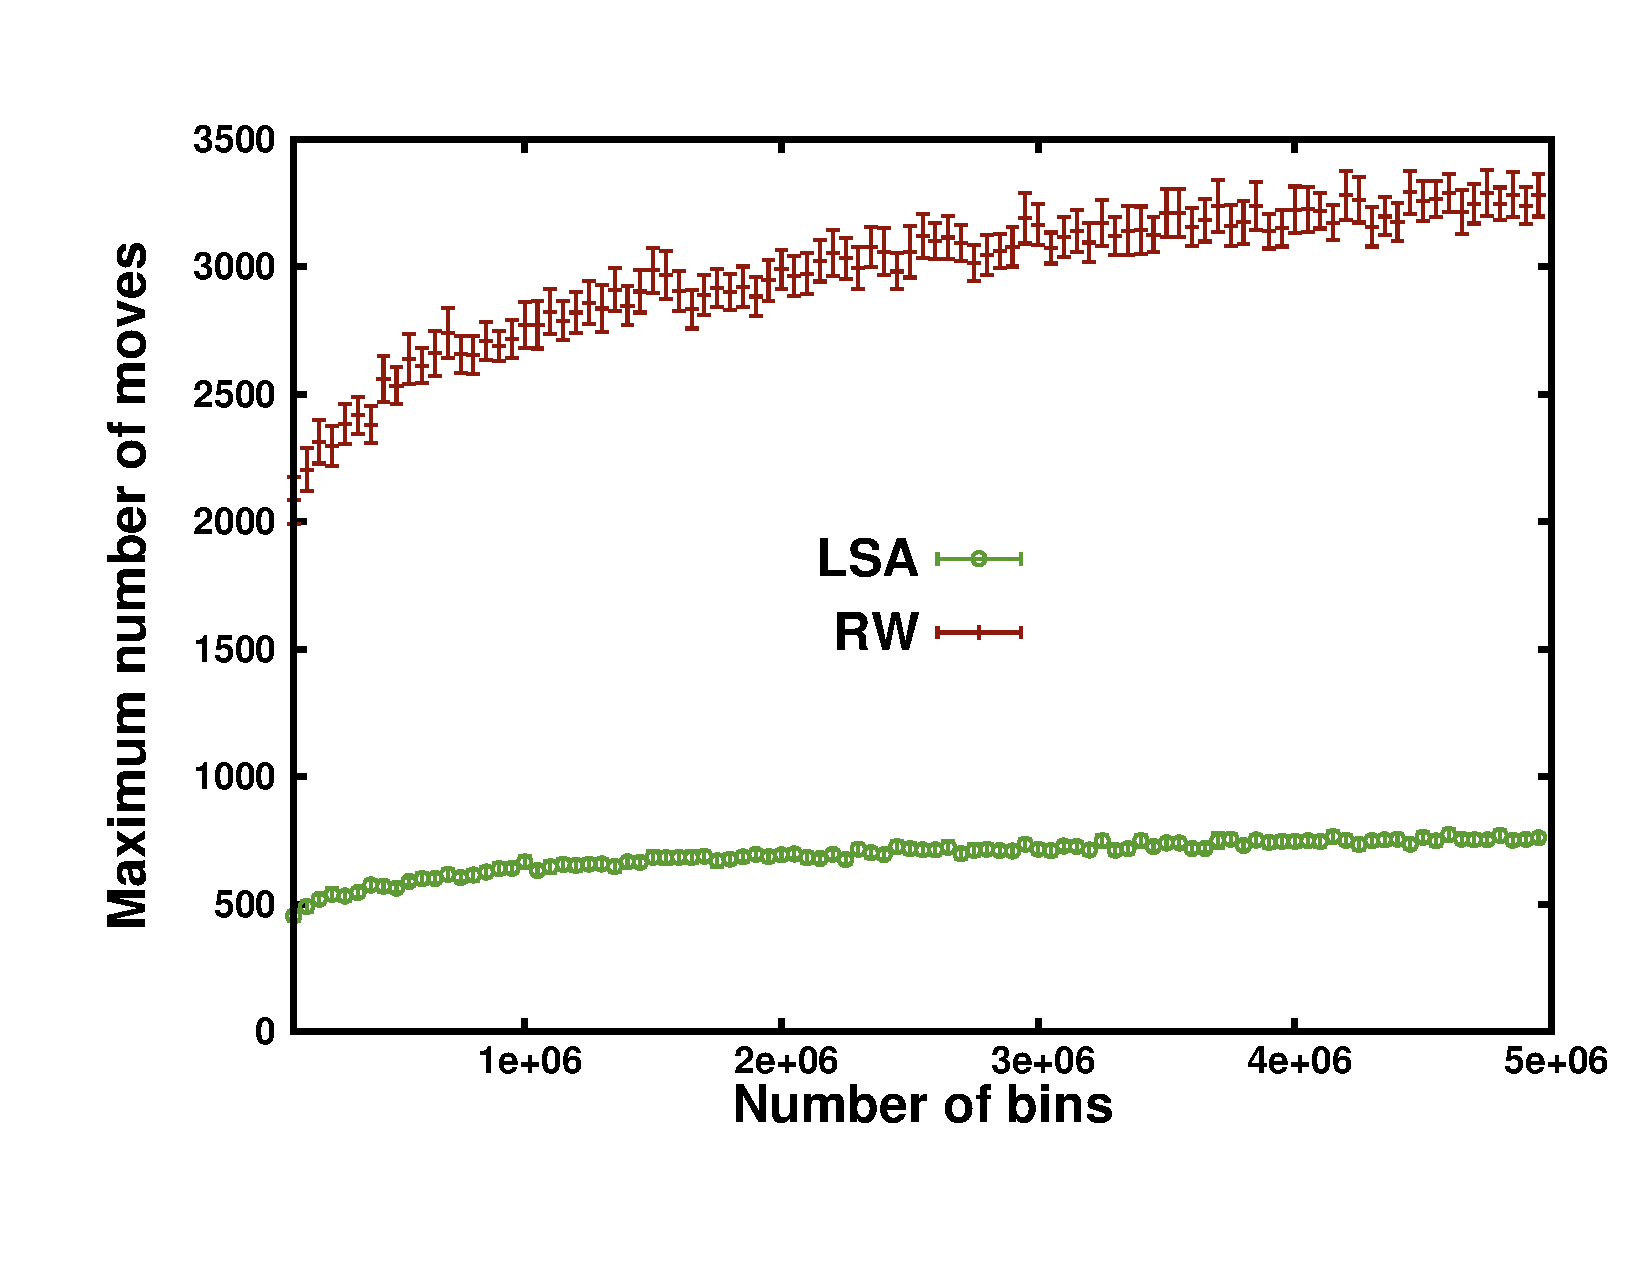
\includegraphics[width=0.45\textwidth]{max-3.pdf}}
   \quad
 \subfigure[$k=4$, $c=0.97 ~(c^*_4\approx 0.976)$.]{\label{fig:his to-3}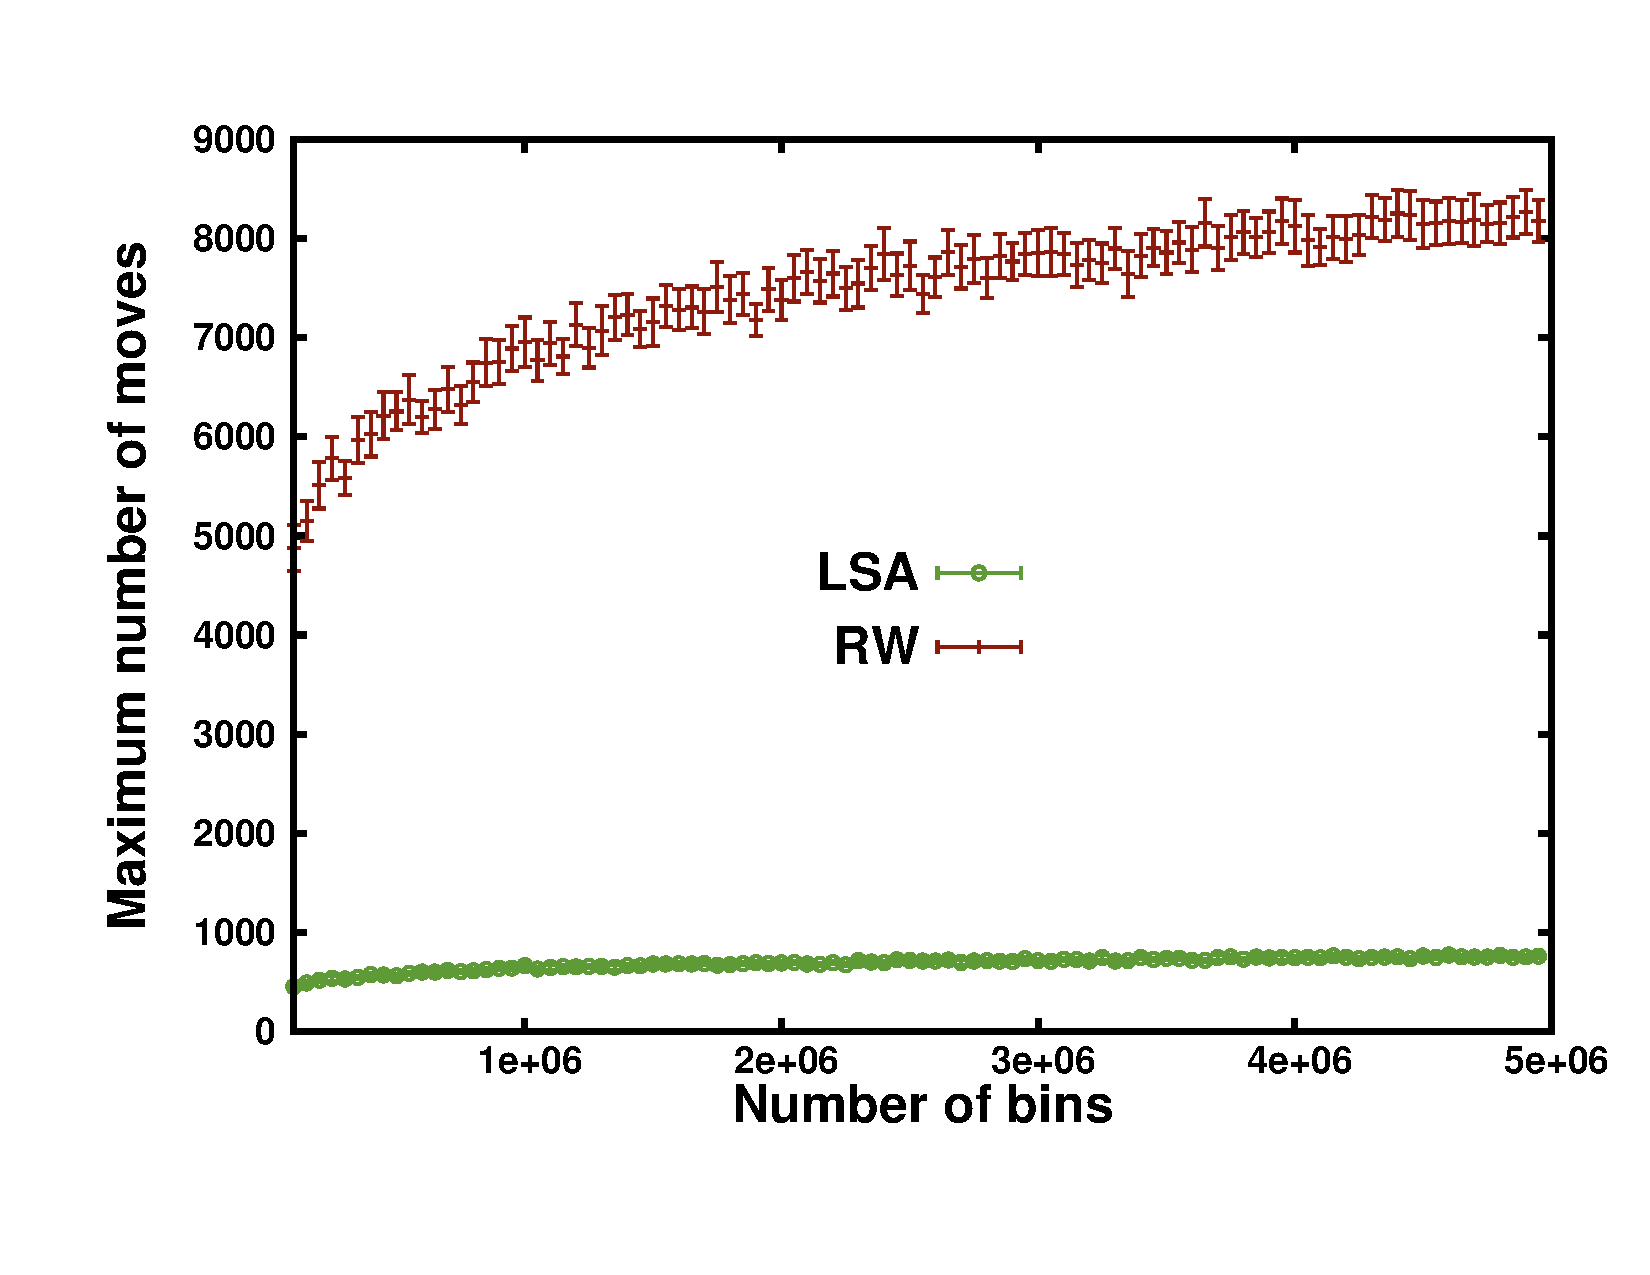
\includegraphics[width=0.45\textwidth]{max-4.pdf}}
   \vspace{-8pt}
   \caption{Comparison of maximum number of moves performed by local search and random walk methods}
    \label{fig:2}
\end{figure*}
\begin{figure*}[h!]
   \centering  
     \subfigure[$k=3$, $c\le 0.915 ~(c^*_3\approx 0.917)$]{\label{fig:fix-3}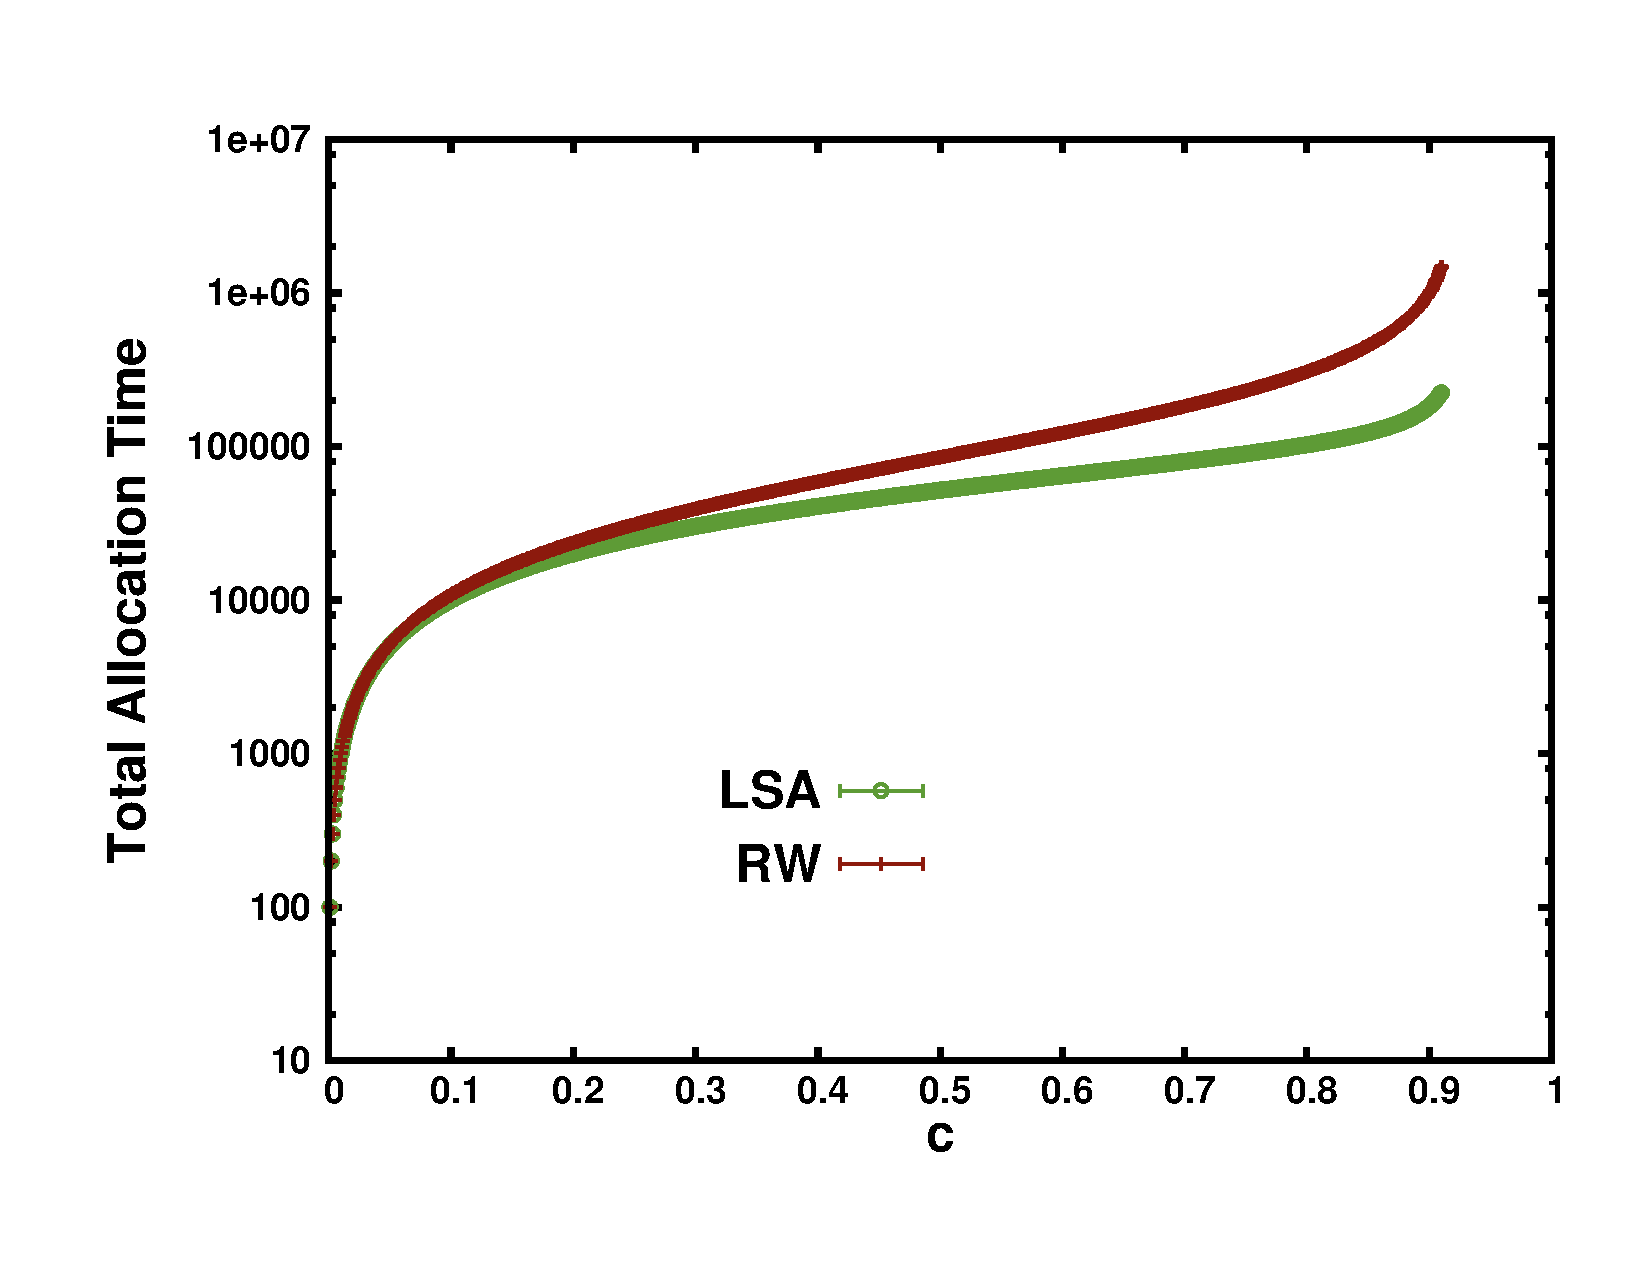
\includegraphics[width=0.45\textwidth]{totald-3.pdf}}
   \quad
       \subfigure[$k=3$, $c\le0.915 ~(c^*_3\approx 0.917)$] {\label{fig:fix-3-total}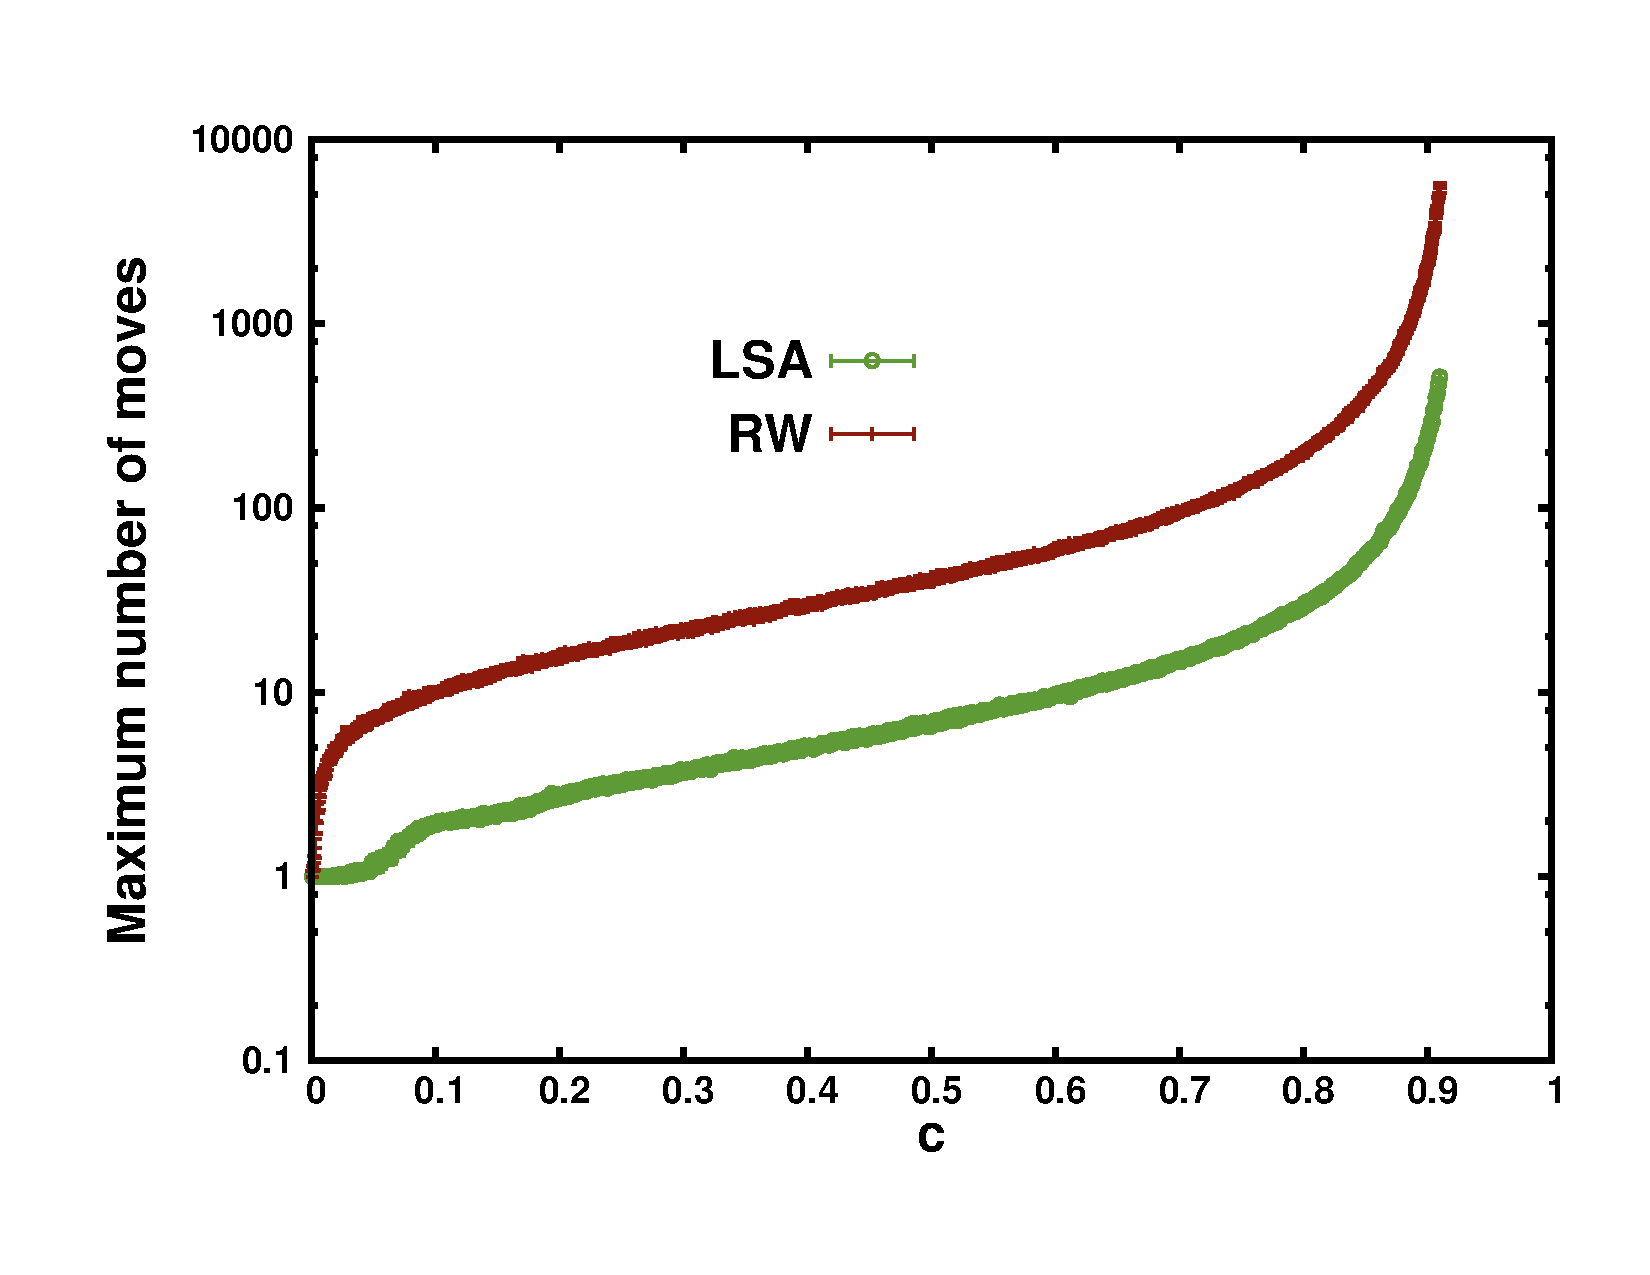
\includegraphics[width=0.45\textwidth]{maxd-3.pdf}}
       \vspace{-8pt}
   \caption{ Comparison of total number of moves and maximum number of moves (for fixed number of locations, $n=10^5$) performed by local search and random walk methods when density c approaches $c^*_k$.}
      \vspace{-1pt}
   \label{fig:3}
\end{figure*}
\begin{figure}[h!]
   \centering  
    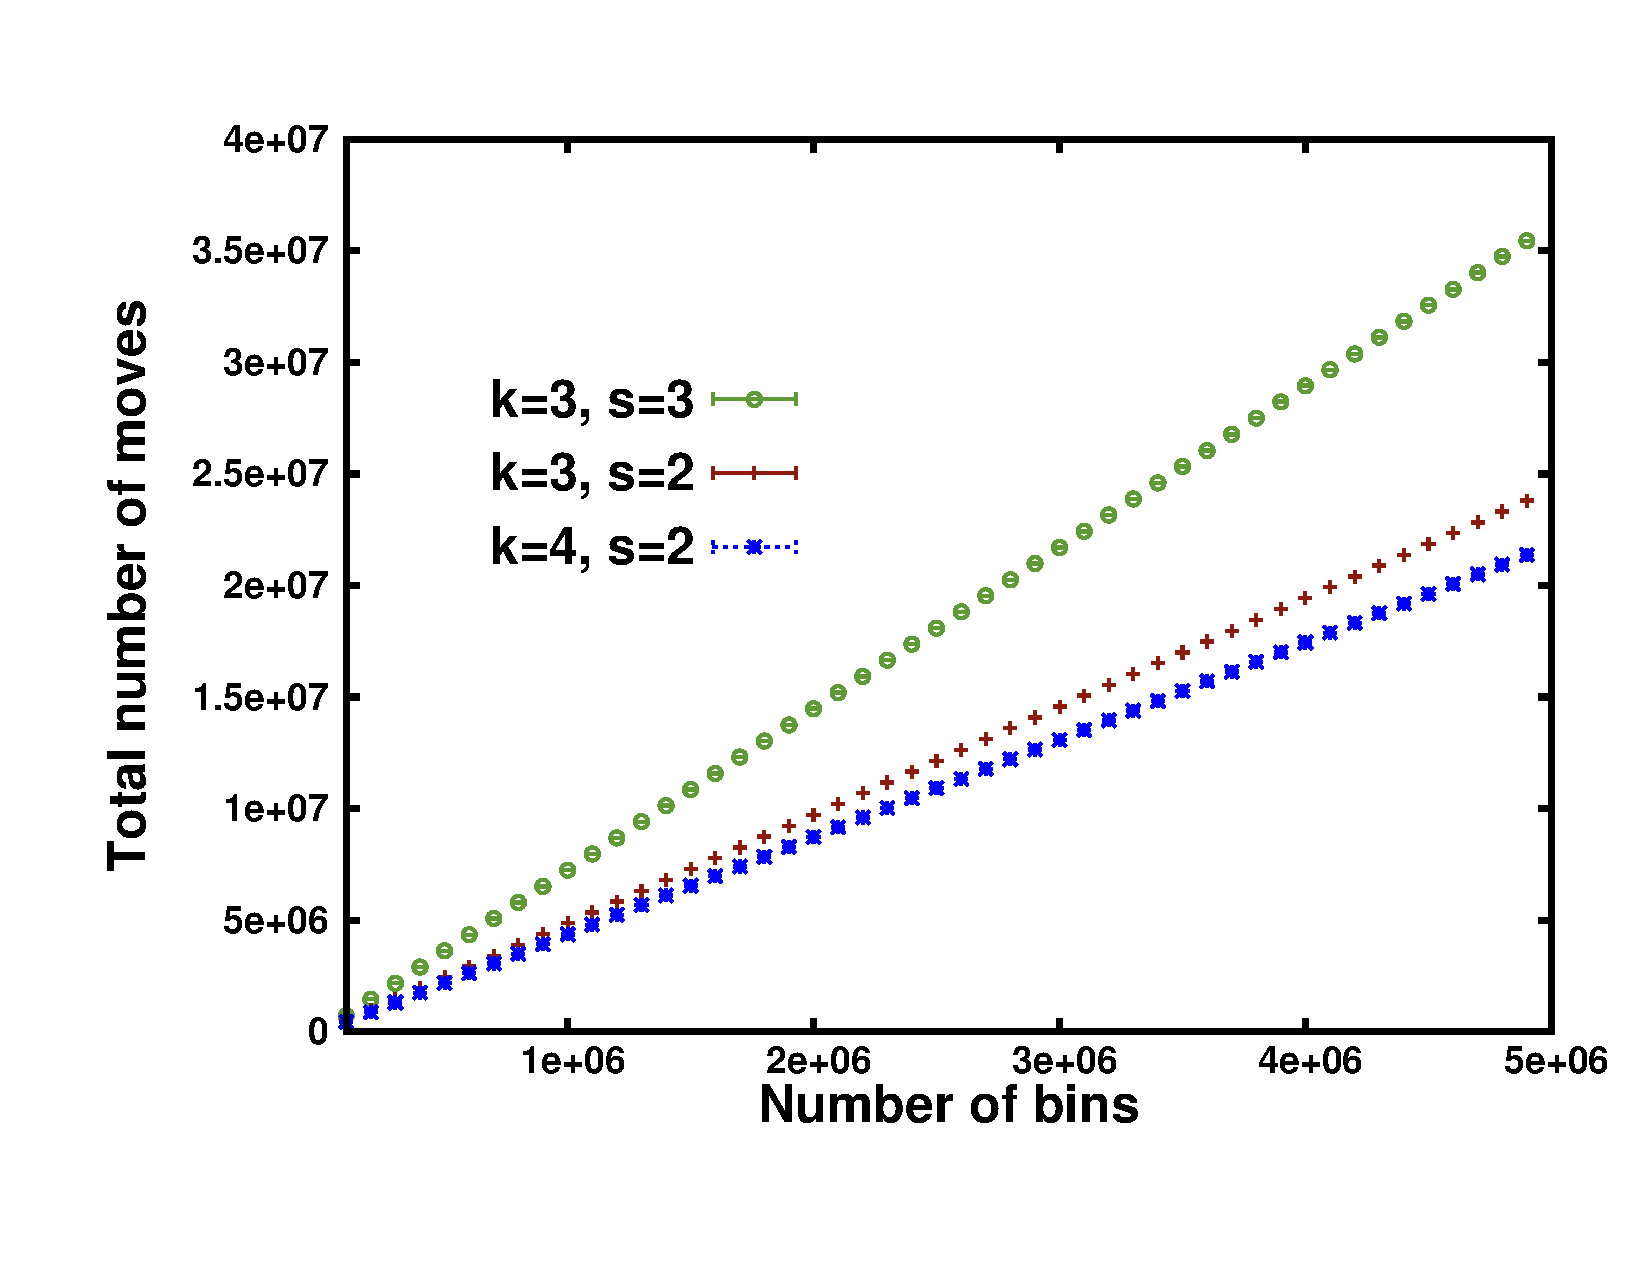
\includegraphics[width=0.85\textwidth]{totalGen-3-2.pdf}
    \caption{Total number of moves for the case where bin capacities (maximum load, $s$) is greater than 1.}
    \label{fig:totalGen}
    \end{figure}

We remark that local search allocation has some additional cost, i.e., the extra space required to store the labels. Though this space is $O(n)$, local search allocation is still useful for the applications where the size of objects (representing the items) to be allocated is much larger than the labels which are integers. Moreover, with high probability, the maximum label of any vertex is $O(\log n)$. Many integer compression methods~\cite{inp:sgl10} have been proposed for compressing small integers and can be potentially useful in our setting for further optimizations. Also in most of the load balancing problems, the speed of finding an assignment is a much desired and the most important requirement.
\begin{algorithm}[h!]
\caption{AssignBall ($x, \mathbf{L},\mathbf{T}$)}
\label{algo:orientEdgegen}
\begin{algorithmic}[1]
\STATE Choose an item $v$ among the $k$ choices of $x$ with minimum label $L(v)$.
\IF{$(L(v)>=n-1)$ }
\STATE $\mathbf{EXIT}$  ~~~~~~~~~~~~~~~~~~~~~~~ $\rhd${\textbf{Allocation does not exist}}
\ELSE
\IF{$({\textsc{Items}}(v)> s-1)$ }
\STATE $L(v) \leftarrow 1+ \min{(L(u)| u \neq v \text{~and $u \in x$})}$
\ENDIF
\IF{$(\textsc{Items}(v)==s )$}
\STATE Choose an item (call it b) randomly from the $s$ items in v
\STATE $y\leftarrow b$~~~~~~~~~~~~~~~~~~ $\rhd${\textbf{Move that replaces an item}}
\STATE Place $x$ in $v$
\STATE $\mathbf{CALL}$ {AssignBall($y, \mathbf{L},\mathbf{T}$)}
\ELSE  
\STATE Place $x$ in $v$ ~~~~~~~~~~~~~~~~~~ $\rhd${\textbf{Move that places an item}}
\ENDIF
\ENDIF
\end{algorithmic}
\end{algorithm}
We also consider the case when each location can hold more than one item. To adapt LSA for this setting we make a small change, i.e., the label of a vertex (location) stays 0 until it is fully filled. Algorithm~\ref{algo:orientEdgegen} gives the modified procedure for the general location capacities. Here {\sc{Items}}$(v)$ gives the number of items already placed in $v$. Let the location capacity or maximum load allowed be $s$. Figure~\ref{fig:totalGen} suggests that the total number of moves are linear in the number of locations for the cases $k=3,4$ where the maximum location capacity is greater than $1$.


\begin{table*}[ht!]
\centering
\footnotesize
\begin{tabular}{@{}l l l l @{}}
\toprule
%\hline \noalign{\smallskip}
\multicolumn{1}{l}{} & Limit on Moves                  & Wall-clock times     & Result Size  \\
\hline \noalign{\smallskip}
LSA        &   1      & 12    & 1029449  \\
       &   2      & 12    & 1080006  \\
        &   4      & 12    & 1082199  \\
        &   5      & 16    & 1082214  \\
        &   10      & 15    & 1082214  \\
        &   50     & 15    & 1082214  \\
        &   100     & 15    & 1082214  \\
        &   1000     & 15    & 1082214  \\
        &   10000    & 27    & 1082214  \\
        &   100000    & 136    & 1082214  \\
        &   $n$    & 1887    & 1082214  \\
\midrule

Hopcroft-Karp                &  & 12605 & 1082214 \\
%\hline \noalign{\smallskip}

\hline \noalign{\smallskip}
\end{tabular}
\caption{Performance of LSA on \textsf{Delicious} dataset. Time is measured in seconds.}
\label{table:softlabel}
\end{table*}

\subsection{Performance on Real-world graphs}

Next, we compare our runtime performance to the optimal algorithm proposed by Hopcroft et al.~\cite{hopcroft1973n}. In this experiment we want to study the effect of number of allowable moves on (a) the actual wall-clock times , (b) the result quality in terms of the size, or number of edges, of the final matching produced (refer Figure~\ref{table:softlabel}). We selected the following representative realworld dataset for our experiments:

\begin{itemize}
  \item \textsf{Delicious dataset : } The \textsf{Delicious} dataset spans nine years from 2003 to 2011 and contain about 340 mio. bookmarks, 119 mio. unique URLs, 15 mio. tags and 2 mio. users~\cite{zubiaga2013harnessing}. Each bookmarked URL is time stamped and tagged with word descriptors. The nodes in one of the sets are URLs and in the other are its corresponding bookmarks.

  % \item \textsf{Yahoo Ad dataset : } Computational advertising used bi-partite graph matching algorithms for its ad placement decisions. 
\end{itemize}

We first observe that the optimal result in the \textsf{Delicious} dataset, i.e. 1082214, is already obtained when the limit on the allowable moves is only five and in 12 seconds. Interestingly, as we increase the limit on the allowable moves, the runtime does not change showing that only a small of defections are sufficient to arrive at an optimal result. However, at higher limits, indeed other permutations are explored (in this case unsuccesfully) resulting in increased runtimes. In any case when the limit is set to $n$, that would guarantee optimality, we still perform an order of magnitude faster than the optimal algorithm of Hopcroft-Karp. 




